We begin with the time-dependent, isotropic scattering slab geometry, S$_N$ transport equations with an isotropic source.
\begin{multline}
    \label{eq:sn_nte}
    \frac{1}{v} \frac{\partial \psi_{m}(x,t)}{\partial t} + \mu_m \frac{\partial \psi_{m}(x,t)}{\partial x} + \Sigma(x) \psi_{m}(x,t) 
     = \frac{1}{2} \left( \Sigma_{s}(x) \sum\limits_{n=1}^N w_n \psi_{n}(x,t) + Q(x,t) \right) \;, \\
    \qquad \qquad m=1, \ldots, N \;, \qquad t > 0 \;, \qquad x \in [0,X]
\end{multline}
where $\psi$ is the angular flux, $t$ is time, $x$ is location, $v$ is speed, $\Sigma$ is the macroscopic total cross-section, $\Sigma_s$ is the macroscopic scattering cross-section, $w_m$ is angular quadrature weight, $\mu_m$ is the angular quadrature ordinate, $m$ is the quadrature index, $N$ is the quadrature order, and $Q$ is the isotropic material source.
The initial and boundary conditions are prescribed angular flux distributions:
\begin{equation*}
    \psi_{m}(x,0) = \psi_{init,m}(x), \qquad m=1 \ldots N \;,
\end{equation*}
\begin{equation*}
    \psi_{m}(0,t) = \psi_{inc,m}^+(t), \qquad \mu_m >0 \;,
\end{equation*}
\begin{equation*}
    \psi_{m}(X,t) = \psi_{inc,m}^-(t), \qquad \mu_m <0 \;.
\end{equation*}

We discretize these equations in time using multiple balance~\cite{variansyah_robust_2021}, which solves two coupled sets of equations. 
First is a backward Euler step (transport equation integrated over a time step):
\begin{subequations}
\begin{multline}
\frac{1}{v} \left( \frac{\psi_{m,k+1/2}(x) - \psi_{m,k-1/2}(x)}{\Delta t} \right) + \mu_m \frac{\partial \psi_{m,k}(x)}{\partial x} + \Sigma(x) \psi_{m,k}(x) \\
= \frac{1}{2} \left(  \Sigma_{s}(x) \sum\limits_{n=1}^N w_n \psi_{n,k}(x) + Q_{k}(x) \right) \;,
\end{multline}
and the second is a balance like auxiliary equation from the multiple balance principle:
\begin{multline}
\frac{1}{v} \frac{\psi_{m,k+1/2}(x) - \psi_{m,k}(x)}{\Delta t/2} + \mu_m \frac{\partial \psi_{m,k+1/2}(x)}{\partial x} + \Sigma(x) \psi_{m,k+1/2}(x) \\
= \frac{1}{2} \left( \Sigma_{s}(x) \sum\limits_{n=1}^N w_n \psi_{n,k+1/2}(x) + Q_{ k+1/2}(x) \right) \;,
\end{multline}
\end{subequations}
where $\Delta t$ is the time step size, $k$ indicates time-average quantities, and $k\pm1/2$ indicates time-edge quantities.
Then, we discretize in space using simple corner balance, which involves a spatial integration over the right and left halves of a spatial cell:
\begin{subequations}
\label{eq:scb-mb}
\begin{multline}
\label{eq:scb-mb-a}
\frac{\Delta x_j}{2} \frac{1}{v} \left( \frac{\psi_{m,k+1/2,j,L} - \psi_{m,k-1/2,j,L}}{\Delta t} \right)
 + \mu_m \left[ \frac{\left( \psi_{m,k,j,L} + \psi_{m,k,j,R} \right)}{2}  - \psi_{m,k,j-1/2} \right] \\
+ \frac{\Delta x_j}{2} \Sigma_{j} \psi_{m,k,j,L} 
= \frac{\Delta x_j}{2} \frac{1}{2} \left( \Sigma_{s,j} \sum\limits_{n=1}^N w_n \psi_{n,k,j,L} + Q_{k,j,L} \right) \;,
\end{multline}  
\begin{multline}
\label{eq:scb-mb-b}
\frac{\Delta x_j}{2} \frac{1}{v} \left( \frac{\psi_{m,k+1/2,j,R} - \psi_{m,k-1/2,j,R}}{\Delta t} \right) +
\mu_m \left[ \psi_{m,k,j+1/2} - \frac{\left( \psi_{m,k,j,L} + \psi_{m,k,j,R} \right)}{2}   \right] \\
+ \frac{\Delta x_j}{2} \Sigma_{j} \psi_{m,k,j,R} = \frac{\Delta x_j}{2} \frac{1}{2} \left( \Sigma_{s,j} \sum\limits_{n=1}^N w_n \psi_{n,k,j,R} + Q_{k,j,R} \right) \;,
\end{multline}  
\begin{multline}
\label{eq:scb-mb-c}
\frac{\Delta x_j}{2} \frac{1}{v} \left( \frac{\psi_{m,k+1/2,j,L} - \psi_{m,k,j,L}}{\Delta t/2} \right) \\
+ \mu_m \left[ \frac{\left( \psi_{m,k+1/2,j,L} + \psi_{m,k+1/2,j,R} \right)}{2}  - \psi_{m,k+1/2,j-1/2} \right]
+ \frac{\Delta x_j}{2} \Sigma_{j} \psi_{m,k+1/2,j,L} \\
= \frac{\Delta x_j}{2} \frac{1}{2} \left( \Sigma_{s,j} \sum\limits_{n=1}^N w_n \psi_{n,k+1/2,j,L} + Q_{k+1/2,j,L} \right) \;,
\end{multline}    
\begin{multline}
\label{eq:scb-mb-d}
\frac{\Delta x_j}{2} \frac{1}{v} \left( \frac{\psi_{m,k+1/2,j,R} - \psi_{m,k,j,R}}{\Delta t/2} \right) + \\
\mu_m \left[ \psi_{m,k+1/2,j+1/2} - \frac{\left( \psi_{m,k+1/2,j,L} + \psi_{m,k+1/2,j,R} \right)}{2}   \right]
+ \frac{\Delta x_j}{2} \Sigma_{j} \psi_{m,k+1/2,j,R} \\
= \frac{\Delta x_j}{2} \frac{1}{2} \left( \Sigma_{s,j} \sum\limits_{n=1}^N w_n \psi_{n,k+1/2,j,R} + Q_{k+1/2,j,R} \right) \;,
\end{multline} 
\end{subequations}
where $\Delta x$ is the cell width, $j$ is the spatial cell index, $L/R$ is the left or right half cell, respectively.
These equations contain the first of the two simple spatial closures---the angular flux at the cell midpoint is a simple average of the two half-cell average quantities:
\begin{subequations}
\begin{equation}
  \psi_{m,k}(x_j) =  \frac{\left( \psi_{m,k,j,L} + \psi_{m,k,j,R} \right)}{2} \;,
\end{equation}
\begin{equation}
  \psi_{m,k+1/2}(x_j) =  \frac{\left( \psi_{m,k+1/2,j,L} + \psi_{m,k+1/2,j,R} \right)}{2} \;.
\end{equation}
\end{subequations}
The second closure is an \textit{upstream} prescription for the cell-edge angular flux:
\begin{subequations}
\begin{equation}
  \psi_{m,k,j+1/2} =
  \begin{cases}
  \psi_{m,k,j,R}, & \mu_m > 0, \\
  \psi_{m,k,j+1,L}, & \mu_m < 0 \;,
  \end{cases}
\end{equation}
\begin{equation}
  \psi_{m,k+1/2,j+1/2} =
  \begin{cases}
  \psi_{m,k+1/2,j,R}, & \mu_m > 0, \\
  \psi_{m,k+1/2,j+1,L}, & \mu_m < 0 \;.
  \end{cases}
\end{equation}
\end{subequations}
Figure \ref{fig:stencil} shows the stencil location for angular flux and source terms. 
\begin{figure}[!htb]
    \centering
    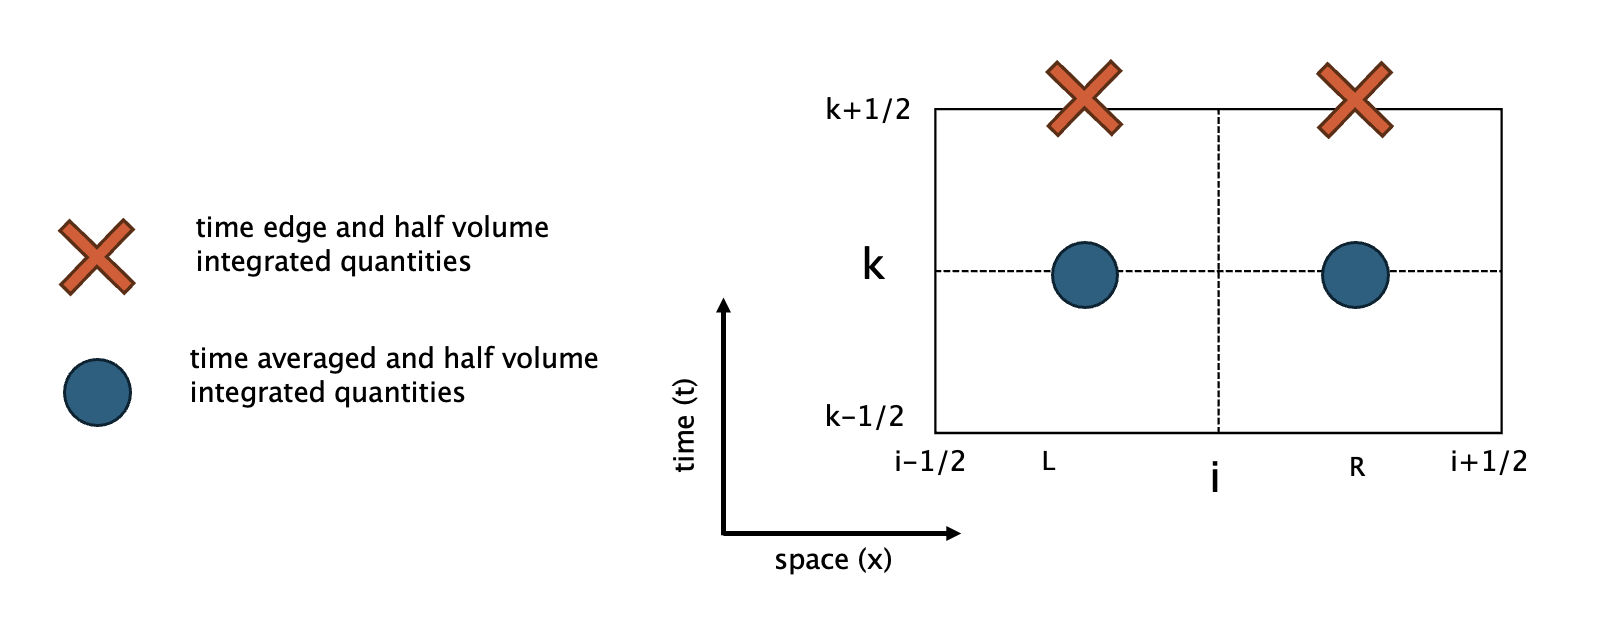
\includegraphics[width=\textwidth]{manuscript2/man2_figs/stencil.png}
    \caption{Discretization stencil for simple corner balance, multiple balance time discretization}
    \label{fig:stencil}
\end{figure}

Solving Eq.~\eqref{eq:scb-mb} iteratively requires operator splitting.
Unknown values (from the current iteration, noted by $l+1$) are moved to the left-hand side to form a large system of linear equations.
In SI, the scalar flux in the scattering source is evaluated at the previous iteration $(l)$, decoupling angles and coupling space.
OCI allows the fluxes incident to the cell---defined by upstream closures---to lag, thus decoupling cells from one another within an iteration.

In OCI, the scattering source is subtracted to the left-hand side and  prior iteration values are employed for all information incident on cell $j$ (moved to the right-hand side).
This means that all $4N$ angular fluxes ($N$ angles at $L$ and $R$, $k$ and $k+1/2$) are computed simultaneously in cell $j$.
This yields a linear system for each cell $j$:
\begin{equation}
    \label{eq:oci}
    \left( \bm{L}_{c,j} - \bm{S}_j \right) \Psi_j^{(l+1)} = -\textbf{L}_{b,j} \Psi_j^{(l)} + \textbf{Q} \;, 
\end{equation}
where $l$ is the iteration index.
The right-hand side can be combined into a known vector
\begin{equation}
     \left( \bm{L}_{c,j} - \bm{S}_j \right) \Psi_j^{(l+1)}  = \bm{b}_j \; ,
\end{equation}
where $\bm{L}_{c,j}$ and $\bm{S}_j$ are both of size $4N\times4N$ and likewise $\bm{b}_j$ is a vector of length $4N$.
\newcommand{\lcmj}[1]{\begin{bmatrix} \bm{L}_{c,j,#1} \end{bmatrix} }
\newcommand{\zeros}{\begin{bmatrix} 0 \end{bmatrix} }
The within-cell operator is
\begin{subequations}
\begin{equation}
    \label{eq:Aja}
    \bm{L}_{c,j} = \begin{bmatrix}
        \lcmj{1} &  &  &  &  \\
          & \ddots  &  &  & \\
          &  & \lcmj{m} &  & \\
          &  &  & \ddots &  \\
          &  &  &  & \lcmj{N}
    \end{bmatrix} \;,
\end{equation}
with zeros elsewhere, where
\begin{equation} \bm{L}_{c,j,m} =
    \label{eq:Aj}
    \begin{bmatrix}
    \frac{|\mu_m| + \Delta x_j \Sigma_{j} }{2}  & \frac{\mu_m}{2} & \frac{\Delta x_j}{2 v \Delta t} & 0 \\
    - \frac{\mu_m}{2} & \frac{|\mu_m| +  \Delta x_j \Sigma_{j,g} }{2} & 0 & \frac{\Delta x_j}{2 v \Delta t} \\
    -\frac{\Delta x_j}{v \Delta t}  & 0 & \frac{\Delta x_j}{v \Delta t} + \frac{|\mu_m| + \Delta x_j \Sigma_{j,g} }{2}  & \frac{\mu_m}{2}  \\
    0 &  -\frac{\Delta x_j}{v \Delta t}  &  - \frac{\mu_m}{2} & \frac{\Delta x_j}{v \Delta t}+ \frac{|\mu_m| + \Delta x_j \Sigma_{j,g}}{2}  \\
    \end{bmatrix} \; .
\end{equation}
\end{subequations}
The right-hand side is
\begin{subequations}
\begin{equation}
    \bm{b}_j =  \left[
    \bm{b}_{j,1} \; \bm{b}_{j,2} \; \cdots \; \bm{b}_{j,N} \right]^{T} \;.
\end{equation}
As the linear system in each cell contains contributions from all angles (both positive and negative) $b_{j,m}$ is given by
\begin{equation} 
    \bm{b}_{j,m} = 
    \begin{cases}
        \bm{b}_{j,m}^+ & \mu_m>0 \\
        \bm{b}_{j,m}^- & \mu_m<0 \\
    \end{cases} \;,
\end{equation}
where
\begin{equation}
     \bm{b}_{j,m}^+ = \begin{bmatrix}
     \frac{\Delta x_j}{4} Q_{k,j,L} + \frac{\Delta x_j}{2 v \Delta t} \psi_{m,k-1/2,j,L} + \mu_m \psi^{(l)}_{m,k,j-1,R} \\
     \frac{\Delta x_j}{4}Q_{k,j,R} + \frac{\Delta x_j}{2 v \Delta t} \psi_{m,k-1/2,j,R} \\
     \frac{\Delta x_j}{4}Q_{k+1/2,j,L} + \mu_m \psi^{(l)}_{m,k+1/2,j-1,R} \\
     \frac{\Delta x_j}{4} Q_{k+1/2,j,R} 
    \end{bmatrix} \;,
\end{equation}
and
\begin{equation}
    \bm{b}_{j,m}^- = \begin{bmatrix}
    \frac{\Delta x_j}{4}  Q_{k,j,L} + \frac{\Delta x_j}{2 v \Delta t} \psi_{m,k-1/2,j,L}  \\
    \frac{\Delta x_j}{4}  Q_{k,j,R} + \frac{\Delta x_j}{2 v \Delta t} \psi_{m,k-1/2,j,R} - \mu_m \psi^{(l)}_{m,k,j+1,L}  \\
    \frac{\Delta x_j}{4}  Q_{k+1/2,j,L}  \\
    \frac{\Delta x_j}{4}  Q_{k+1/2,j,R} - \mu_m \psi^{(l)}_{m,k+1/2,j+1,L}
    \end{bmatrix} \;.
\end{equation}
\end{subequations}
The elements of the ${S_j}$ matrix are defined by
\begin{equation}
    \label{eq:scatter}
   [\mathbf{S}_j]_{k.l} = \begin{cases}
			\frac{\Delta x_j \Sigma_{s,j}}{4}w_{|(l-k)|/3)}, & \text{if $\mod{\frac{(l-k)}{3} =0}$}\\
            0, & \text{otherwise}
		 \end{cases} \; ,
%  \frac{\Delta x_j \Sigma_{s,j}}{4} w_n \;
\end{equation}
where $w$ are the angular quadrature weights.
%To adapt this scheme to anisotropic scattering regimes alterations to $S_j$ would be required.
Finally,
\begin{subequations}
\begin{equation}
\Psi^{(l+1)}_j =  \begin{bmatrix}
    \bm{\psi}_{j,1}^{(l+1)}, \;
    \bm{\psi}_{j,2}^{(l+1)}, \;
    \cdots \;
    \bm{\psi}_{j,N}^{(l+1)}
    \end{bmatrix} ^{T} \; ,
\end{equation}
where
\begin{equation} 
\bm{\psi}_{j,n}^{(l+1)} = \begin{bmatrix}
    \psi_{n,k,j,L}^{(l+1)}, \;
    \psi_{n,k,j,R}^{(l+1)}, \;
    \psi_{n,k+1/2,j,L}^{(l+1)}, \;
    \psi_{n,k+1/2,j,R}^{(l+1)}
    \end{bmatrix}^{T} \;.
\end{equation}
\end{subequations}
One-cell inversion iterations continue until
\begin{equation}
    ||\Psi^{(l+1)}-\Psi^{(l)}||_{2} < \epsilon(1-\rho_e) \; ,
\end{equation}
where $\epsilon$ is the convergence tolerance and
\begin{equation}
    \rho_e = \frac{||\Psi^{(l+1)}-\Psi^{(l)}||_{2}}{||\Psi^{(l)}-\Psi^{(l-1)}||_{2}}
\end{equation}
is an empirical estimation of the spectral radius computed at every iteration of a transport solve.
After convergence, the time-step counter increments and the time-step process can be repeated.

Generally, Jacobi and Gauss--Seidel iterations converge faster when a system is more diagonally dominant \cite{isaacson_numerical_1966, golub_matrix_1983}.
Equation~\eqref{eq:Aj} contains ($ \delta/2 = \Delta x\Sigma/2 $) on the diagonals.
So in the thin limit (when $\delta\rightarrow 0$) the system becomes overall less diagonally dominant and converges more slowly.
However Equation~\eqref{eq:Aj} also involves $\Delta x/(v\Delta t)$ terms in elements (3,3) and (4,4).
Thus, a smaller time step will cause the system to become more diagonally dominant.
We provide a similar description of simple corner balance and multiple balance time discretization for an unpreconditioned source iteration \cite{morgan2023oci}.
